\title{
	
\includegraphics[width=0.3\textwidth]{tum_logo} \\[0.6em]
	Signed Distance Field Ray Differentials}
\author{	
        Kevin Galim \\
        TUM---Technical University of Munich\\
        Boltzmannstrasse 3, 85748 Garching, Germany
}
\date{\today}

\documentclass[12pt]{article}

\usepackage[backend=biber]{biblatex}
\DeclareSourcemap{  
	\maps[datatype=bibtex]{
		\map{
			\step[fieldset=url, null]
			\step[fieldset=doi, null]
			\step[fieldset=isbn, null]
			\step[fieldset=issn, null]
		}                   
	}
}


\addbibresource{VoxelGI.bib}

\usepackage{amsmath}
\usepackage{amssymb}
\usepackage{graphicx}
\usepackage{float}
\usepackage{mathtools}
\usepackage{multirow}
\usepackage{rotating}
\usepackage{booktabs}
\usepackage{array}
\usepackage{subcaption}
\usepackage[width=0.9\textwidth]{caption}

\DeclarePairedDelimiter\abs{\lvert}{\rvert}%
\DeclarePairedDelimiter\norm{\lVert}{\rVert}%

\newcommand{\halfvalue}[1]{\frac{#1}{2}}
\newcommand{\halfpow}[1]{^\frac{#1}{2}}
\newcommand{\pardiff}[2]{\frac{\partial #1}{\partial #2} }
\newcommand{\pardiffsqsame}[2]{\frac{\partial^2 #1}{\partial #2^2} }
\newcommand{\pardiffsq}[3]{\frac{\partial^2 #1}{\partial #2 \partial #3} }
\newcommand{\pardiffx}[1]{\frac{\partial #1}{\partial x} }
\newcommand{\pardiffy}[1]{\frac{\partial #1}{\partial y} }
\newcommand{\newlinel}{\\[0.3em]}
\newcommand{\newlinell}{\\[0.6em]}

\newcolumntype{C}[1]{>{\centering\arraybackslash} m{#1}}
\newcommand*\rot{\rotatebox[origin=c]{90}}

% results
\newcommand{\testscreenres}{512x512}
\newcommand{\testlowres}{64}
\newcommand{\testhighres}{512}
\newcommand{\testimage}[1]{\includegraphics{images/results/#1}}

\DeclareMathOperator{\Hessian}{Hess}
\DeclarePairedDelimiter\floor{\lfloor}{\rfloor}

% Ray Differential Equations
\newcommand{\transferp}{
	P' = P + tD}
\newcommand{\transferd}{
	D' = D}
\newcommand{\transferdpdx}{
	\pardiff{P'}{x} = \left( \pardiff{P}{x} + t \pardiff{D}{x} \right) + \pardiff{t}{x} D}
\newcommand{\transferdddx}{
	\pardiff{D'}{x} = \pardiff{D}{x}}

\newcommand{\reflectionp}{
	P' = P}
\newcommand{\reflectiond}{
	D' = D - 2(D \cdot N) N}
\newcommand{\reflectiondpdx}{
	\pardiff{P'}{x} = \pardiff{P}{x}}
\newcommand{\reflectiondddx}{
	\pardiff{D'}{x} = \pardiff{D}{x} - 2 \left( (D \cdot N) \pardiff{N}{x} + \pardiff{(D \cdot N)}{x} N \right)}

\newcommand{\refractionp}{
	P' = P}
\newcommand{\refractiond}{
	\begin{aligned}
		&D' = \eta D - \mu N \\
		&\mu = \left( \eta (D \cdot N) - (D' \cdot N) \right) \\
		&D' \cdot N = -\sqrt{1 - \eta^2 \left( 1 - (D \cdot N)^2 \right) }
	\end{aligned}}
\newcommand{\refractiondpdx}{
	\pardiff{P'}{x} = \pardiff{P}{x}}
\newcommand{\refractiondddx}{
	\pardiff{D'}{x} = \eta \pardiff{D}{x} - \left( \mu \pardiff{N}{x} + \pardiff{\mu}{x} N \right)}


%\setlength{\parindent}{0pt}

\begin{document}
	
\maketitle

\begin{abstract}
Ray differentials allow estimating the pixel footprint in the scene which can be used for filtering and anti-aliasing. This report introduces the use of ray differentials with signed distance functions, functions returning the distance to the closest point of the shape.  
\end{abstract}

\section{Introduction}
Ray tracing is a powerful method for image synthesis and creating realistic looking images. Although this technique works really well for rendering any kind of 3D geometry and lighting can be simulated really realistic, it also suffers from issues regarding that only single rays with no thickness are traced though pixels. This could lead to aliasing if the resolution is not chosen high enough. To address this, supersampling could be used which traces multiple rays through one pixel and combines the results. This, however, comes with a high overhead considering the number of traced rays.

Another interesting approach is ray differentials \cite{Igehy:1999}. This technique tries to estimate the extent of the whole footprint of ray inside the scene by keeping track of the differentials of a ray. The differentials of the ray give the change of the ray's origin and direction when moving it on the x- and y-axis on the image plane. This can be used to determine filter regions and apply filtering in the respective area to consider the whole projected area of a pixel inside the scene.

The main focus for ray differentials are triangle meshes which are commonly used for rendering. An alternative approach of scene representation are signed distance fields which are useful for high detailed objects and exact representation of objects \cite{jones:2006}. Here the shape is not represented as vertices connected to triangles, but as a mathematical function giving the distance to surface of the shape.

\section{Ray Differentials}
\subsection{Definition}
Using ray differentials, the footprint of a ray in the scene can be estimated. The basic concept is to regard an image plane ray as a function depending on the x and y offset on the image plane
\begin{equation}
R = P + tD 
\qquad
R(x,y) = \left\{ P(x,y) \quad D(x,y) \right\}
.\end{equation}
To keep track of the ray change when shifting it on x- and y-direction on image plane, the ray function can be partially differentiated by the image plane coordinates x and y
\begin{equation}
\pardiff{R}{x} = \left\{ \pardiff{P}{x} \quad \pardiff{D}{x} \right\}
\qquad
\pardiff{R}{y} = \left\{ \pardiff{P}{y} \quad \pardiff{D}{y} \right\}
.\end{equation}
By calculating these differentials for every ray propagation, the position and direction change of the ray when shifting on the image plane can be computed on every position along the ray path. This change rate can then be used to estimate the footprint extent of the pixel where the ray is shot through (Figure \ref{fig:raydiff}). For the differentiated ray, any arbitrary neighbor ray can be approximated which allows to approximate footprints into the scene by taking the difference of the approximated neighbor ray and the differentiated ray.

\begin{figure}[h]
	\centering
	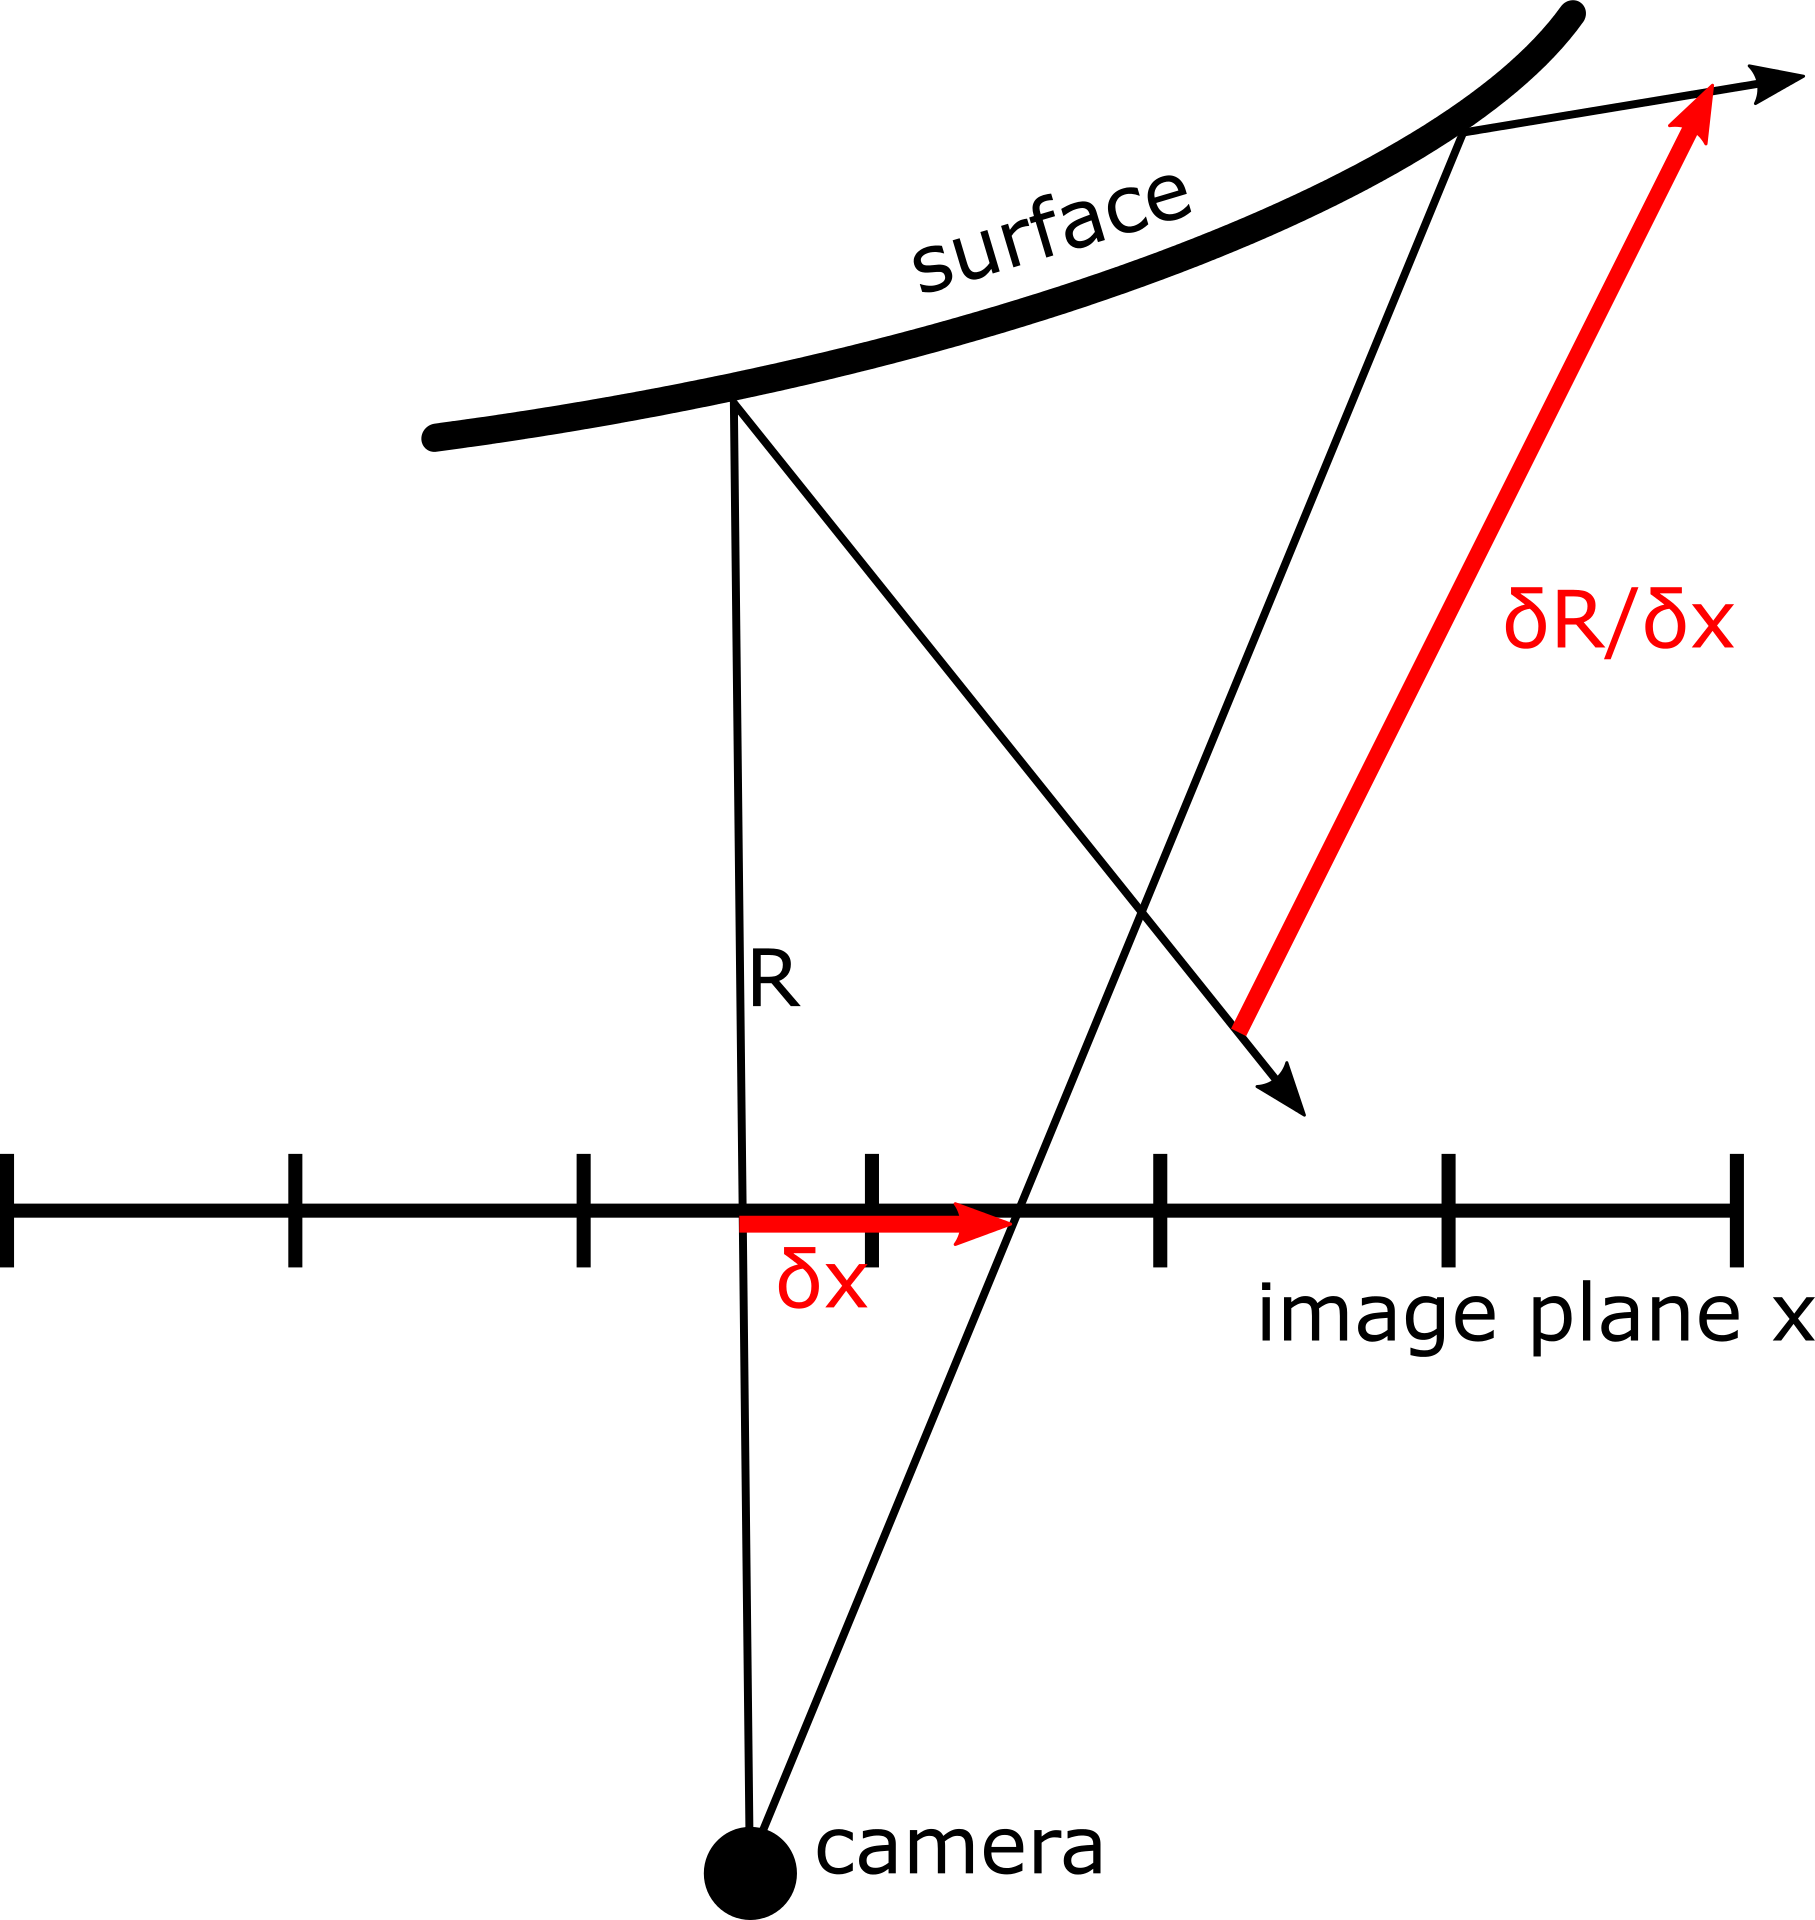
\includegraphics[width=0.4\textwidth]{images/raydiff}
	\caption{Ray Differentials on image plane x-axis.}
	\label{fig:raydiff}
\end{figure}

\subsection{Computation}
Initially, every ray starts at the camera position and is directed through the image plane at coordinate $(x,y)$
\begin{equation}
\begin{aligned}
P(x,y) &= \text{Camera} \\
D(x,y) &= \frac{d}{(d \cdot d) \halfpow{1}} \qquad d(x,y) = \text{View} + x \text{Right} + y \text{Up}
.\end{aligned}
\end{equation}
Differentiation by x then yields the following term
\begin{equation}
\begin{aligned}
\pardiff{P}{x} &= 0 \\
\pardiff{D}{x} &= \frac{(d \cdot d) \text{Right} - (d \cdot \text{Right}) d}{(d \cdot d)\halfpow{3}}
.\end{aligned}
\end{equation}
Differentiating by y would give a similar term.

For every change in position or direction by propagation, e.g. reflection and refraction, there is an equation to update the ray position and direction which can be again partially differentiated by x and y to update the ray differentials as well. Table \ref{table:raydiff} shows a quick overview of common ray operations and their derivate. For more details, see chapter 3.1 of "Tracing Ray Differentials" \cite{Igehy:1999}.

\begin{table}[H]
\centering
\resizebox{0.98\textwidth}{!}{
	\begin{tabular}{ C{3mm} l  l }
		\toprule
		& Operation      & Derivative \newlinel
		\midrule
		\multirow{2}{*}{\rotatebox[origin=c]{90}{Transfer}} & $\transferp$ & $\transferdpdx$ \\[0.8em]
		& $\transferd$ & $\transferdddx$ \\[0.8em]
		\midrule
		\multirow{2}{*}{\begin{sideways}Reflection\end{sideways}} & $\reflectionp$ & $\reflectiondpdx$ \\[0.8em]
		& $\reflectiond$ & $\reflectiondddx$ \\[0.8em]
		\midrule
		\multirow{2}{*}{\begin{sideways}Refraction\end{sideways}} & $\refractionp$ & $\refractiondpdx$ \\[0.8em]
		& $\refractiond$ & $\refractiondddx$ \\[0.8em]
		\bottomrule
	\end{tabular}}
	\caption{Updating ray differentials for common ray propagation operations. The left column shows how ray position and direction gets updated with the specific ray operation. The right column shows the exact same update for the derivate of the ray position and direction in x direction.}
	\label{table:raydiff}
\end{table}

\section{Signed Distance Fields}
\subsection{General Signed Distance Fields}
The idea of a signed distance field of a shape $S$ is a function which takes a 3D point in world space as input and yields a scalar value giving the minimal distance of the point to the closest surface of the shape. Generally the value of the signed distance function is negative if the point is inside the shape, 0 on the shape and positive outside of the shape.
\begin{equation} \label{eq:sdfdef}
SDF(P) = 
\begin{cases} 
-\text{distance}(P, S_{surface})  & \mbox{if } \text{$P$ inside shape $S$} \\ 
0 & \mbox{if } \text{$P$ on the surface of shape $S$} \\
\text{distance}(P, S_{surface})  & \mbox{if } \text{$P$ outside shape $S$} \\ 
\end{cases}
\end{equation}
The surface of the shape is then defined as the set of points where the signed distance function yields 0.
\begin{equation}
S_{surface} = \{P \in \mathbb{R}^3 \mid SDF(P) = 0\}
\end{equation}
For proper rendering, the definition of the surface by this function is not sufficient. On every surface point, a normal has to be defined for lighting and ray propagation like reflection and refraction. When dealing with signed distance fields, the normal at a surface point is equivalent to the value of the gradient of the signed distance function at that point \cite{Osher:2003}.
\begin{equation} \label{eq:sdfnormal}
n = \nabla SDF \qquad N = \frac{n}{(n \cdot n) \halfpow{1}} 
\end{equation}

\subsection{Discrete Signed Distance Fields}
\subsubsection{Storing and evaluating the SDF}
Since it is difficult to compute a specific continuous signed distance function describing the current scene, a discrete function can be used. This function can be seen as a discrete and uniform 3D grid over the cartesian coordinate system of the scene. Each grid vertex in the field stores the closest signed distance of the vertex to the surface of the scene. 

The function, however, needs to be evaluated for any point in the continuous space, not only on points stored in the 3D field. In order to get the signed distance at an arbitrary point $P$, an interpolation is performed between the stored signed distance values of the function in the neighborhood of point $P$. The most common way is to use trilinear interpolation by linearly interpolating between the 8 vertices in the neighborhood of $P$ \cite{calakli:2011}.

\subsubsection{Field Interpolation}
A more general approach is to model the interpolation and determination of the signed distance at an arbitrary point $P$ by applying an 1D filter kernel $f$ over the 3D field neighborhood of $P$. 
\begin{equation}
f(v_1, \dots, v_n, t)
\end{equation}
This filter function with width $n$ and takes $n$ values and interpolates among them based on the filter weight $t \in [0, 1]$. 
A linear filter kernel for example would look like
\begin{equation}\label{eq:linearint}
f(v_1, v_2, t) = (1 - t) v_1 + t v_2
.\end{equation}
In order to filter with a 1D kernel in the 3D field, a neighborhood of $n^3$ vertices around $P$ is selected, resulting in a cube of vertices with size $n$. Using this area, the 1D kernel is applied $n^2$ times over all vertices in x direction. Over this resulting square of values, the kernel is applied $n$ times over the vertices in y direction resulting in $n$ values. Over these final values in z direction the kernel is applied once which gives the final interpolation value. Formulating as function, we get
 
\begin{equation} \label{eq:intfunc}
v(V, t) = f
\begin{pmatrix}
f 
\begin{pmatrix}
f(v_{111}, \dots, v_{n11}, t_x), \\
\vdots \\
f(v_{1n1}, \dots, v_{nn1}, t_x), \\
t_y
\end{pmatrix}, \\
\vdots \\
f
\begin{pmatrix}
f(v_{11n}, \dots, v_{n1n}, t_x), \\
\vdots \\
f(v_{1nn}, \dots, v_{nnn}, t_x), \\
t_y
\end{pmatrix}, \\[2.5em]
t_z
\end{pmatrix}
.\end{equation}
$v_{xyz} \in V$ denotes the discretely stored signed distance value at index $\{x, y, z\}$ in the neighborhood interpolation area $V$ of $P$. Figure \ref{fig:interpolation} shows $P$ inside the filter area of 8 vertices which is, for example, used for linear interpolation.

\begin{figure}[h]
	\centering
	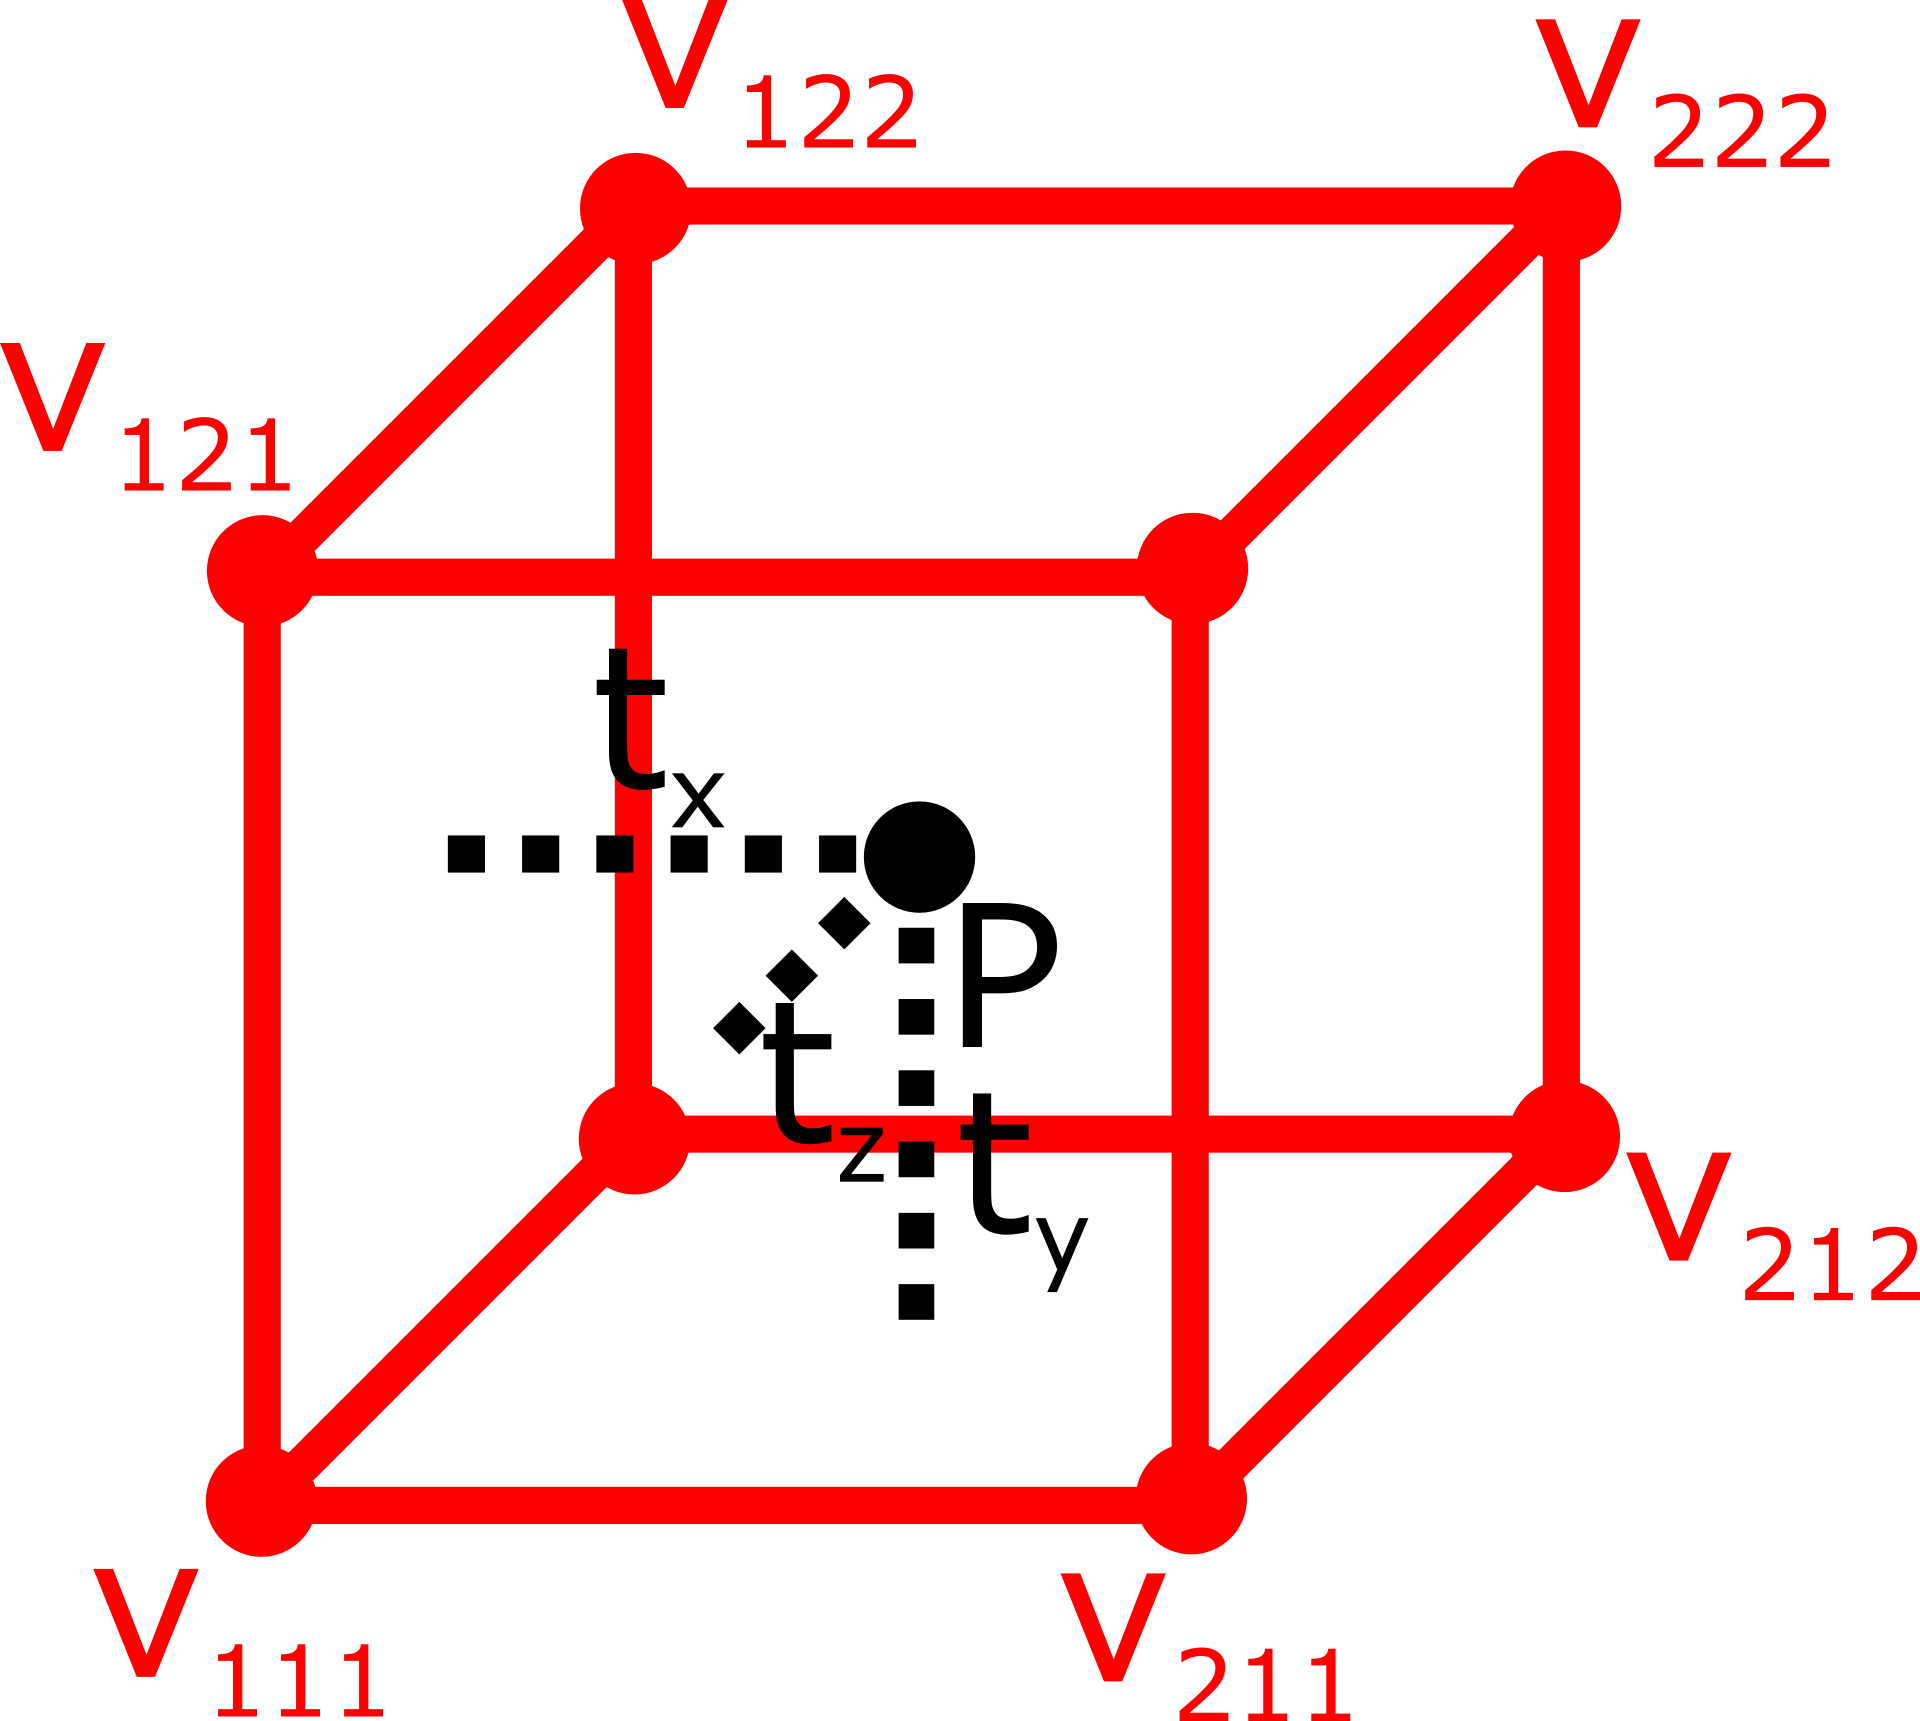
\includegraphics[width=0.4\textwidth]{images/interpolation}
	\caption{Interpolation to determine value at $P$. $v_{111}$ is the lower vertex and $v_{222}$ is the upper vertex of the filter area consisting of a total of 8 vertices. $t$ is the filter weight which is calculated based on the distance to the lower vertex.}
	\label{fig:interpolation}
\end{figure}

\subsection{Building the discrete Signed Distance Function}
\subsubsection{Definition of the discrete Signed Distance Function}
Considering the general definition of signed distance functions \eqref{eq:sdfdef} and interpolation of discrete grid values \eqref{eq:intfunc}, a concrete signed distance function can now be build using these two components.

First of all, it is assumed that the signed distance function takes positions $P$ in world space as input. To determine the neighborhood of $P$ inside the discrete SDF grid and to calculate the filter weight $t$, this position must first be transfered to absolute grid coordinates $P_{\text{grid}}$ (Figure \ref{fig:absgridcoords}). Assuming that the SDF grid in the world coordinate system is centered at $V_{\text{origin}}$ with an extent of $V_{\text{scale}}$ in all 6 axis directions and a grid resolution $V_{\text{resolution}}$, then the absolute grid position can be calculated as
\begin{equation}
P_{\text{grid}} = V_{\text{resolution}} \left(\frac{\left(P - V_{\text{origin}}\right)}{2V_{\text{scale}}}  + \begin{pmatrix}\frac{1}{2} & \frac{1}{2} & \frac{1}{2}\end{pmatrix}^T \right) 
.\end{equation}
The resulting $P_{\text{grid}}$ ranges between $\begin{pmatrix} 0 & 0 & 0\end{pmatrix}^T$ and $V_{\text{resolution}} - \begin{pmatrix} 1 & 1 & 1\end{pmatrix}^T$. A cell in absolute grid space has width $1$. All vertices of the grid storing the SDF values are located on the integer grid positions. To now determine arbitrary signed distance values, interpolation is performed using the appropriate stored neighbor grid values. The vertex values are weighted according to the position of the value to lookup inside the neighborhood. 
\begin{figure}[h]
	\centering
	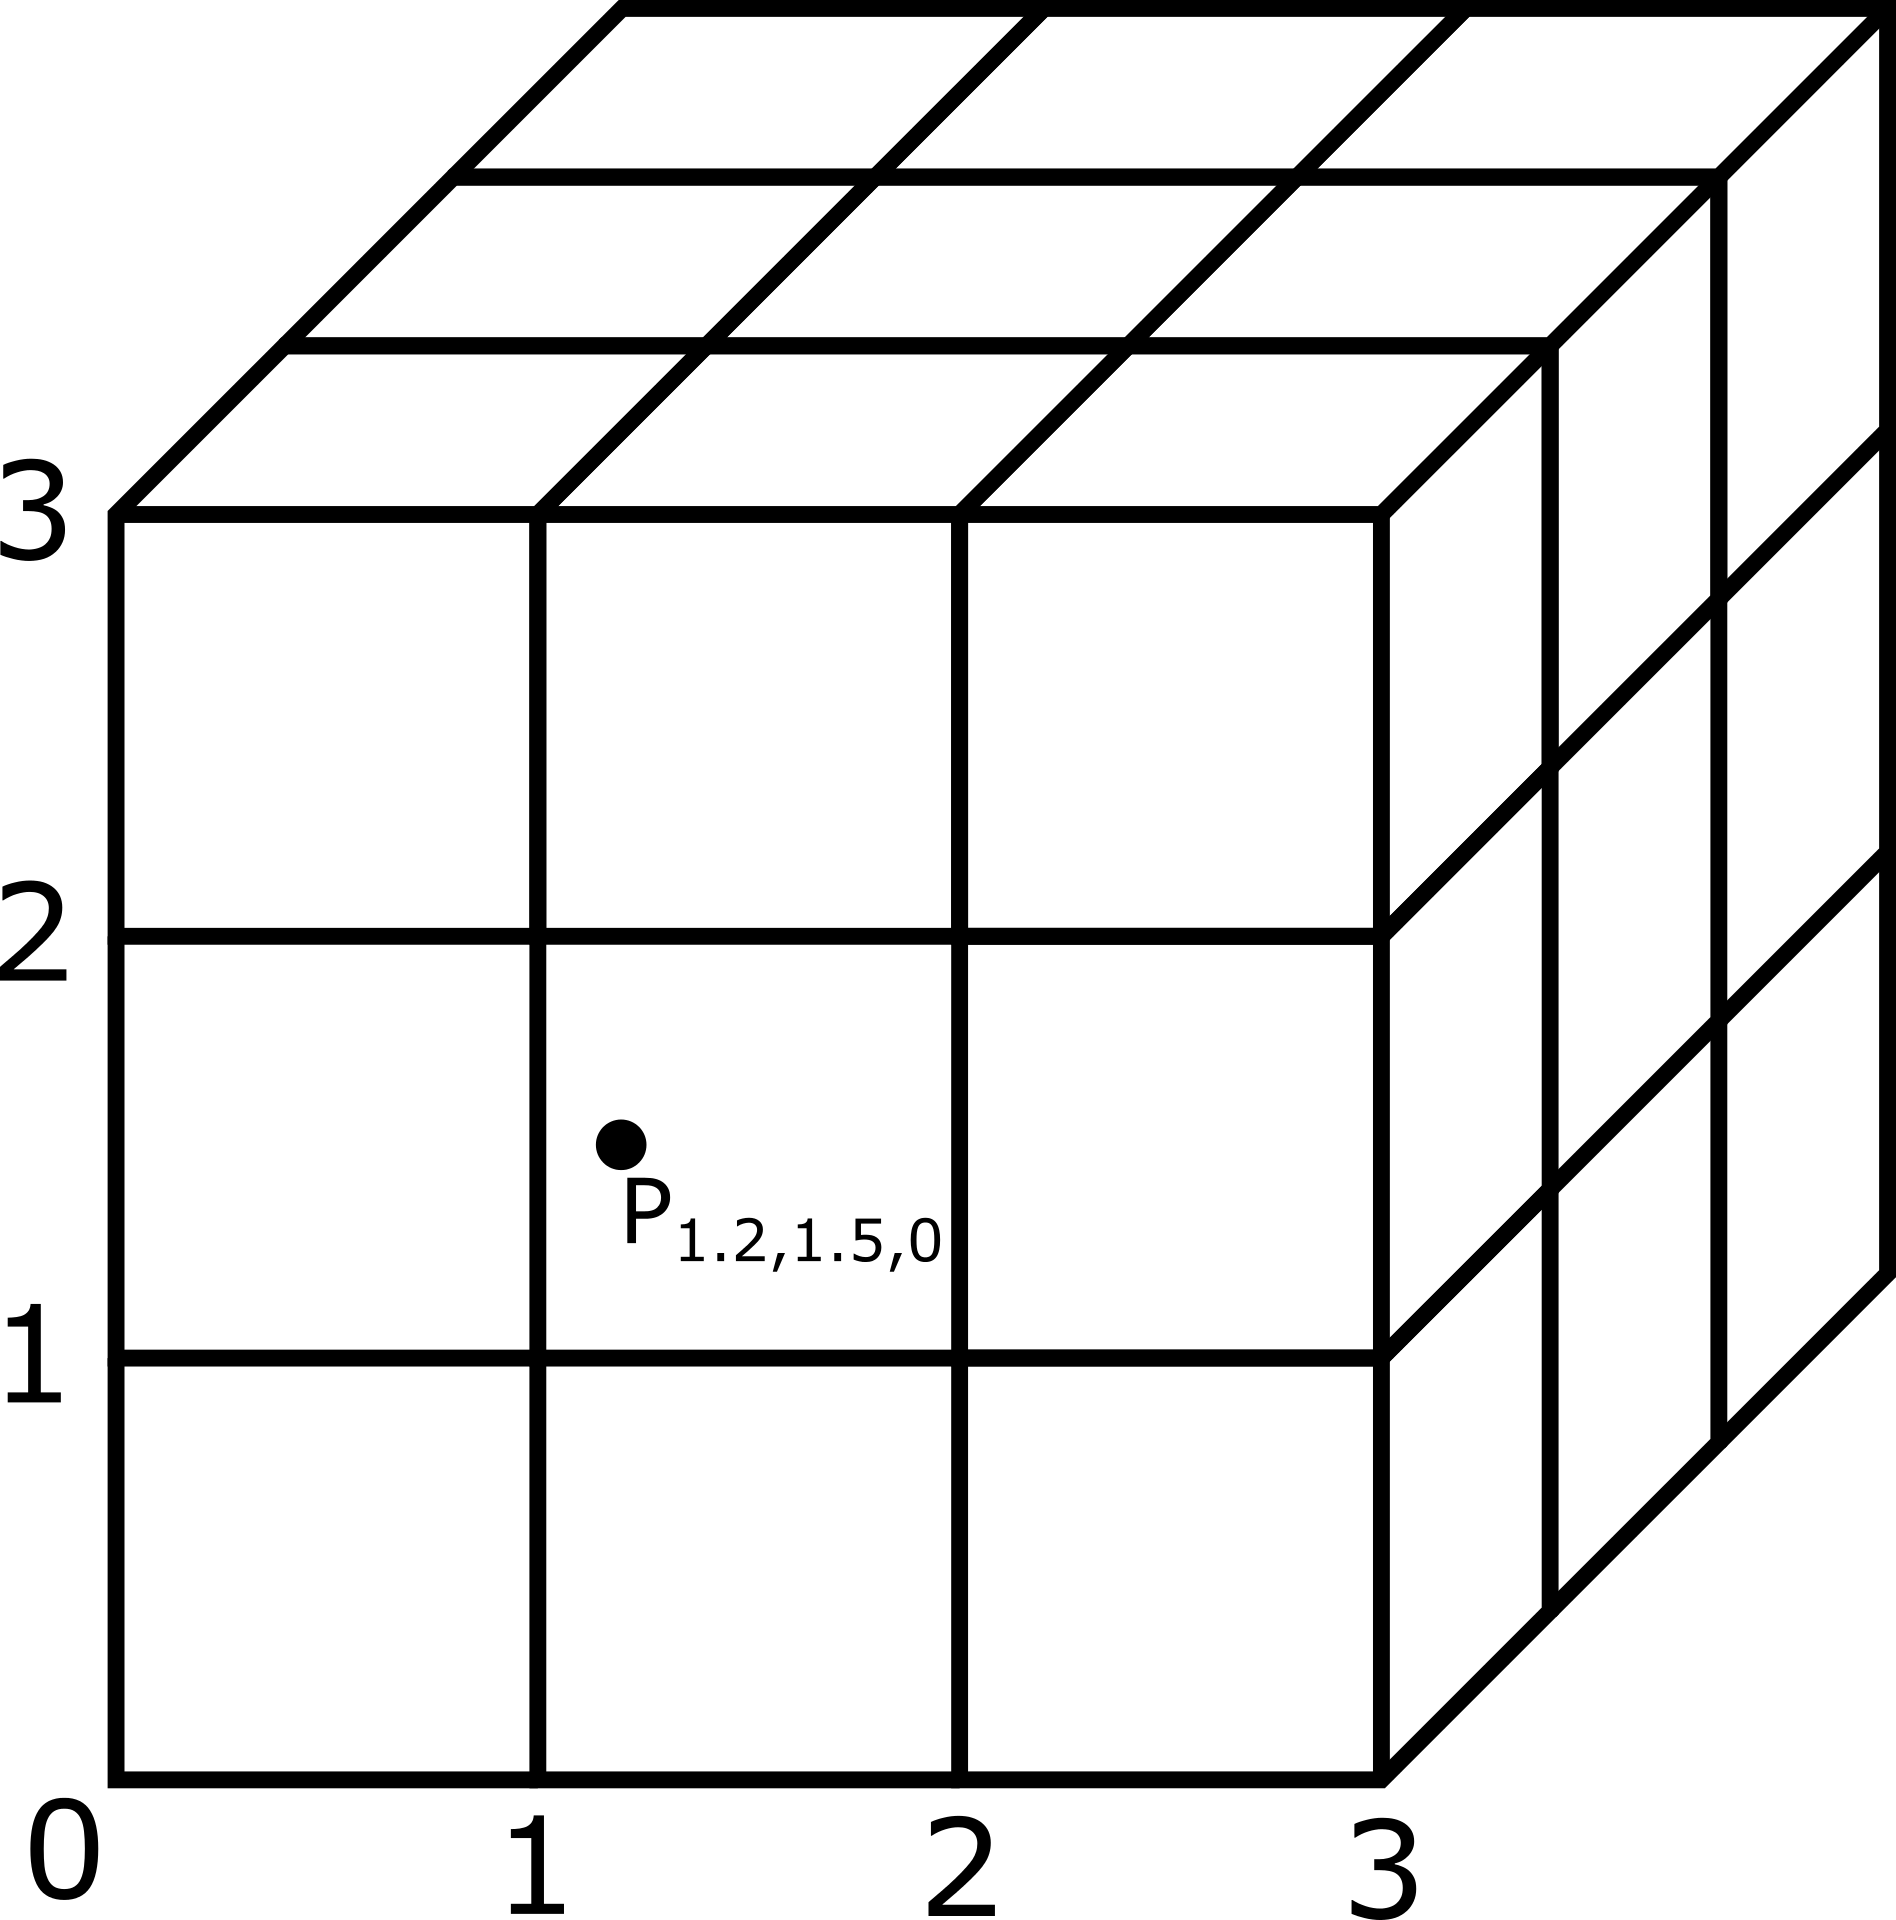
\includegraphics[width=0.4\textwidth]{images/absolute_grid_coords}
	\caption{$P$ in absolute grid coordinates.}
	\label{fig:absgridcoords}
\end{figure}

Thus, a three dimensional filter weight $t$ (Figure \ref{fig:interpolation}) is calculated by taking the distance between $P$ and its nearest lower integer vertex
\begin{equation} \label{eq:weightt}
t = P_{grid} - \floor{P_{grid}}
\end{equation}
$t$ ranges between $\begin{pmatrix} 0 & 0 & 0 \end{pmatrix}^T$ and $\begin{pmatrix} 1 & 1 & 1 \end{pmatrix}^T$. This weight is then used for the interpolation function \eqref{eq:intfunc} to formulate the final discrete signed distance function
\begin{equation} \label{eq:discretesdf}
SDF(P) = v \left(N_{fP}, t \left(P_{\text{grid}}\left(P \right) \right) \right).
\end{equation}
$N_{fP}$ here is the set of values in the neighborhood of $P$ which the filter kernel $f$ interpolates on.

\subsubsection{Definition of the surface normal}
In order to define a normal on the surface of the discrete signed distance function, the gradient has to be determined ($\odot$ stands for the component-wise product of two vectors)

\begin{equation}
n = \nabla SDF = 
\begin{pmatrix}
\pardiff{SDF}{P_x} \newlinell
\pardiff{SDF}{P_y} \newlinell
\pardiff{SDF}{P_z}
\end{pmatrix}
=
\begin{pmatrix}
\pardiff{v}{t_x} \newlinell
\pardiff{v}{t_y} \newlinell
\pardiff{v}{t_z}
\end{pmatrix}
\odot
\begin{pmatrix}
\pardiff{t_x}{P_x} \newlinell
\pardiff{t_y}{P_y} \newlinell
\pardiff{t_z}{P_z}
\end{pmatrix} 
\end{equation}
which results in the component-wise product of the interpolation and the derivate of $t$ for the unnormalized surface normal
\begin{equation} \label{eq:normaldiscrete}
n = \nabla v \odot \pardiff{t}{P}
.\end{equation}
Since the $floor$ function occurs in the definition of $t$ \eqref{eq:weightt}, the derivate $t'$ has singularities at all integer grid points $P_{\text{grid}} \in \mathbb{Z}$. Assuming the SDF grid is axis aligned in the world coordinate system, the differentiation yields
\begin{equation}
\pardiff{t}{P} = \frac{V_{\text{resolution}}}{2V_{\text{scale}}}
\qquad
P_{\text{grid}} \notin \mathbb{Z}
.\end{equation}
However, this derivative is constant and all singularities are removable using its constant value. Thus the singularities can be removed by setting
\begin{equation}
\pardiff{t}{P} := \frac{V_{\text{resolution}}}{2V_{\text{scale}}}
\qquad
P_{\text{grid}} \in \mathbb{Z}
.\end{equation}

\section{Ray Differentials with Signed Distance Fields}
\subsection{Calculating the Normal Differential}
In order to compute the ray differentials, the differential of the surface normal $\pardiff{N}{x}$ has to be calculated to compute the derivate of the ray reflection and refraction (Table \ref{table:raydiff}). The differential in x-direction can be computed as
\begin{equation}
\begin{aligned}
\pardiff{n}{x} &= \pardiff{\left( \nabla SDF \right)}{x} =
\begin{pmatrix}
\pardiffsq{SDF}{P_x}{x} \newlinell
\pardiffsq{SDF}{P_y}{x} \newlinell
\pardiffsq{SDF}{P_z}{x}
\end{pmatrix} \newlinell
&=
\begin{pmatrix}
\pardiffsqsame{v}{t_x}  \left( \pardiff{t_x}{P_x} \pardiff{P_x}{x} \right) \pardiff{t_x}{P_x} +
\pardiffsq{v}{t_x}{t_y} \left( \pardiff{t_y}{P_y} \pardiff{P_y}{x} \right) \pardiff{t_x}{P_x} + 
\pardiffsq{v}{t_x}{t_z} \left( \pardiff{t_z}{P_z} \pardiff{P_z}{x} \right) \pardiff{t_x}{P_x}
\newlinell
\pardiffsq{v}{t_y}{t_x} \left( \pardiff{t_x}{P_x} \pardiff{P_x}{x} \right) \pardiff{t_y}{P_y} +
\pardiffsqsame{v}{t_y}  \left( \pardiff{t_y}{P_y} \pardiff{P_y}{x} \right) \pardiff{t_y}{P_y} +
\pardiffsq{v}{t_y}{t_z} \left( \pardiff{t_z}{P_z} \pardiff{P_z}{x} \right) \pardiff{t_y}{P_y}
\newlinell
\pardiffsq{v}{t_z}{t_x} \left( \pardiff{t_x}{P_x} \pardiff{P_x}{x} \right) \pardiff{t_z}{P_z} +
\pardiffsq{v}{t_z}{t_y} \left( \pardiff{t_y}{P_y} \pardiff{P_y}{x} \right) \pardiff{t_z}{P_z} +
\pardiffsqsame{v}{t_z}  \left( \pardiff{t_z}{P_z} \pardiff{P_z}{x} \right) \pardiff{t_z}{P_z}
\end{pmatrix}
\newlinell
&=
\left(
\begin{pmatrix}
\pardiffsqsame{v}{t_x} & \pardiffsq{v}{t_x}{t_y} & \pardiffsq{v}{t_x}{t_z} \newlinell
\pardiffsq{v}{t_y}{t_x} & \pardiffsqsame{v}{t_y} & \pardiffsq{v}{t_y}{t_z} \newlinell
\pardiffsq{v}{t_z}{t_x} & \pardiffsq{v}{t_z}{t_y} & \pardiffsqsame{v}{t_z}
\end{pmatrix}
\left( \pardiff{t}{P} \odot \pardiff{P}{x} \right) \right) \odot \pardiff{t}{P} \newlinell
\end{aligned}
\end{equation}
which results in the following term for the normal differential in x-direction:
\begin{equation}
\pardiff{n}{x} = \left( \Hessian(v) \left( \pardiff{t}{P} \odot \pardiff{P}{x} \right) \right) \odot \pardiff{t}{P}
\end{equation}
The final step is derive the vector normalization \eqref{eq:sdfnormal} to get the derivate for the normalized normal with length 1:
\begin{equation}
\pardiff{N}{x} = \frac{(n \cdot n) \pardiff{n}{x} - (n \cdot \pardiff{n}{x}) \cdot n}{(n \cdot n) \halfpow{3}}
\end{equation}

\subsection{Choosing the interpolation kernel}
For simplicity and performance reason, linear interpolation is usually used in computer graphics \eqref{eq:linearint}. 
However, the derivate of the linear kernel is constant and yields flat normals when calculating the gradient \eqref{eq:normaldiscrete} which can be a problem for realizing curved shapes (Figure \ref{fig:linvscubnormal}). All values in the same neighborhood, enclosed by the same 8 neighborhood values, are seen as lying on the same flat plane whereby hard edges arise at the border of each neighborhood region . Therefore, choosing a cubic interpolation instead is a reasonable approach. A common cubic interpolation technique are Catmull-Rom splines \cite{twigg:2003}\cite{weston:2002}. The filtering can be expressed as:
\begin{equation}
f(v_1, v_2, v_3, v_4, t) = 
\begin{pmatrix}
1 & t & t^2 & t^3
\end{pmatrix}
\begin{pmatrix}
0 & 1 & 0 & 0 \\
-\tau & 0 & \tau & 0 \\
2 \tau & \tau - 3 & 3 - 2 \tau  & -\tau \\
- \tau & 2 - \tau & \tau - 2 & \tau
\end{pmatrix}
\begin{pmatrix}
v_1 \\
v_2 \\
v_3 \\
v_4
\end{pmatrix}
\end{equation} 
$\tau$ is called "tension" and controls how strong the curve bends at the interpolation points. It is often chosen as $\halfvalue{1}$. This value will also be used in this report.

This filter has a width of 4 and operates on a total of 64 values in 3D space. The interpolation curve always passes through all input values and produces a soft curve among all interpolation data. It yields $v_2$ for $t=0$ and $v_3$ for $t=1$. It can simply be plugged into the 3D kernel interpolation \eqref{eq:intfunc} and act as tricubic interpolation between grid values.

\begin{figure}[h]
	\centering
	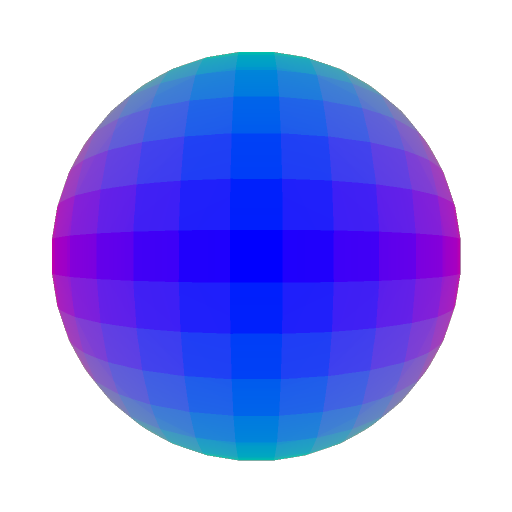
\includegraphics[width=0.25\textwidth]{images/sphere16linear}
	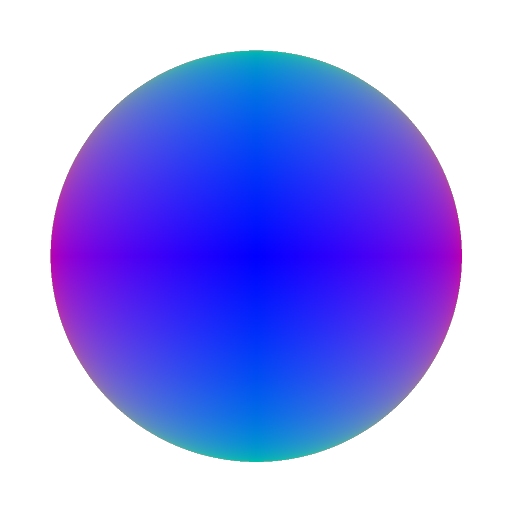
\includegraphics[width=0.25\textwidth]{images/sphere16cubic}
	\caption{Linear and cubic filter. Image shows a sphere with a grid resolution of 16, filtered with a linear filter (left) and a cubic filter (right). Sphere is colored by normals.}
	\label{fig:linvscubnormal}
\end{figure}

\subsection{Texture filtering}
\subsubsection{Texture Coordinate Differentials}
A practical application of ray differentials is texture filtering. To map textures to the signed distance grid, we store additionally a pair of UV coordinates at each grid vertex and interpolate among them similarly to SDF values. A similar expression to \eqref{eq:discretesdf} can be derived for the texture coordinates by taking the UV coordinates instead of the SDF values:
\begin{equation}
T(P) = 
\begin{pmatrix}
v_u \left(N_{fP}, t \left(P_{\text{grid}}\left(P \right) \right) \right) &
v_v \left(N_{fP}, t \left(P_{\text{grid}}\left(P \right) \right) \right)
\end{pmatrix}^T
.\end{equation}
Now this equation can be derived similarly to get the change of the texture coordinate when shifting the ray on the image plane for the x-direction:
\begin{equation}
\pardiff{T}{x} = 
\begin{pmatrix}
\left( \nabla v_u \odot \pardiff{t}{P} \right) \cdot \pardiff{P}{x} &
\left( \nabla v_v \odot \pardiff{t}{P} \right) \cdot \pardiff{P}{x}
\end{pmatrix}^T
\end{equation}
This can now be used to estimate the projection of the pixel onto the texture, the ray footprint, since this describes the change of the texture coordinate when shifting the ray on the image plane in x- and y-direction \cite{Igehy:1999}. By multiplying the differentials by the texel pixel ratio, an estimate about the extent of the footprint in texture space can be calculated
\begin{equation}
\begin{aligned}
\Delta T_x &\approx \pardiff{T}{x} \odot \text{texel}/\text{pixel} \\[0.6em]
\Delta T_y &\approx \pardiff{T}{y} \odot \text{texel}/\text{pixel} \\[0.6em]
T_{\text{size}} &= 
\begin{pmatrix}
\left( \Delta T_x \cdot \Delta T_x \right) \halfpow{1} &
\left( \Delta T_y \cdot \Delta T_y \right) \halfpow{1}
\end{pmatrix}
\end{aligned}
\end{equation}

The texture should now be filtered in the footprint region. A common approach for texture filtering is mipmapping \cite{williams:1983} where the texture gets stored in progressively smaller resolutions. According to an level of detail, a certain texture resolution is then chosen where the texture is finally sampled. The level of detail should be selected regarding the extent of the footprint inside the texture. An algorithm for choosing a suitable level of detail is to take the logarithm of the longer side of the footprint extent.
\begin{equation} \label{eq:lodselect}
\text{LoD} = \log_2 \left( \max \left( T_{\text{size}_x}, T_{\text{size}_y} \right) \right)
\end{equation}
If the LoD lies between two detail representations, linear interpolation is performed between the two textures. 

\subsubsection{Results}
To test the texture filtering, a scene consisting of a reflective sphere and a paper sheet containing text is used. The reflective sphere is placed directly in front of the camera while the paper is placed behind it and not directly visible by the camera, only in the reflection on the sphere. The whole scene is stored inside a signed distance grid with a resolution of either \testlowres{}  or \testhighres{}  in all three dimensions. The scene is rendered using raytracing with a screen resolution of \testscreenres{}. The gradient and hessian matrix for the normal differential are calculated using automatic differentiation \cite{gower:2010}. The effect of mipmapping will be tested as well as the influence of the grid dimension and the interpolation type linear and cubic as presented above.



Figure \ref{fig:testnomipmap} shows the render result of the scene when no mipmapping is applied. The paper reflection in the sphere mirror shows clear aliasing since the footprint of the ray is not considered, only the intersection point of the ray is used. The next test shows the same scene, but this time the mipmapping technique \eqref{eq:lodselect} is used with linear and cubic interpolation at a grid resolution of \testlowres{} (Figure \ref{fig:testlowinterpolation}). Both images show a clear improvement considering texture aliasing although the cubic interpolation here yields superior results. The linear interpolation produces visible flat surfaces on the sphere. Another rendering is performed at the higher grid resolution of \testhighres{} (Figure \ref{fig:testhighinterpolation}). The higher resolution makes the sphere in the linear interpolation test seem more smooth. However, the reflection in the linear result is distorted and not smooth. The cubic result is better and similar to the lower resolution cubic result. The last image (Figure \ref{fig:testssaa}) shows the cubic interpolation with 2x supersampling which produces a small improvement by additional smoothing of the texture.

\begin{figure}[H]
	\centering
	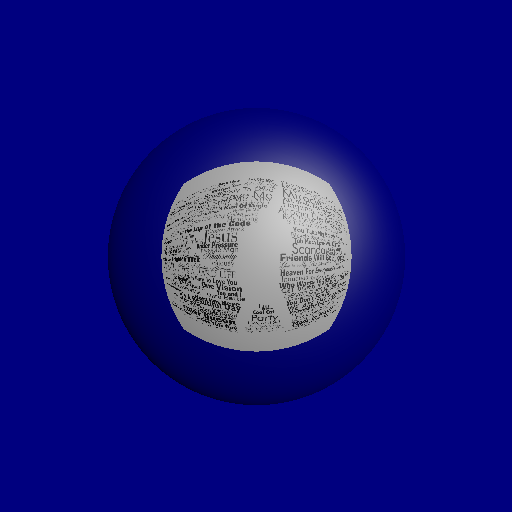
\includegraphics[width=0.6\linewidth]{images/spere_mirror_high_nolod_cubic}
	\caption{Reflective sphere scene without mipmapping, $\testhighres^3$ grid dimension, cubic interpolation.}
	\label{fig:testnomipmap}
\end{figure}

\begin{figure}[H]
	\centering
	\begin{subfigure}[b]{0.49\linewidth}
		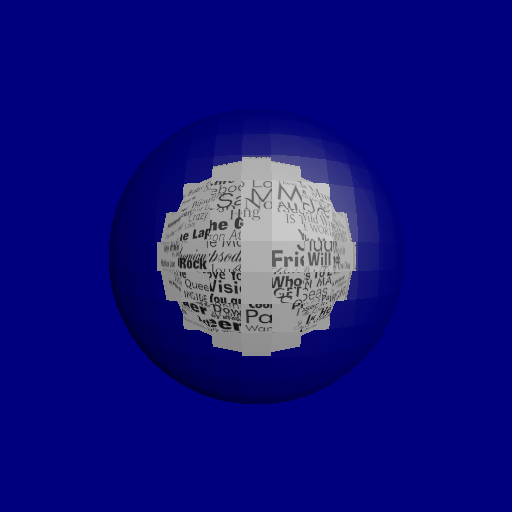
\includegraphics[width=\linewidth]{images/spere_mirror_low_lod_linear}
		\caption{Linear Interpolation.}
	\end{subfigure}
	\begin{subfigure}[b]{0.49\linewidth}
		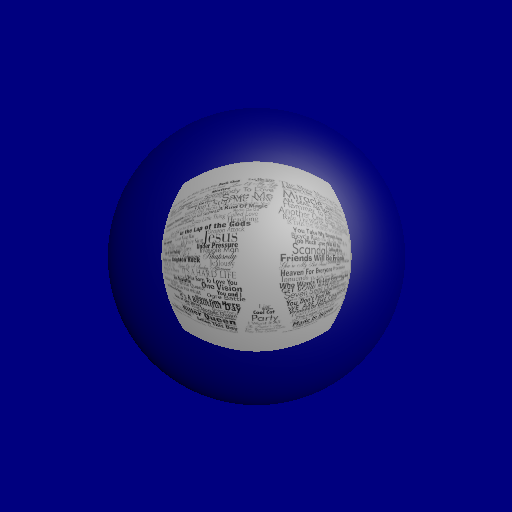
\includegraphics[width=\linewidth]{images/spere_mirror_low_lod_cubic}
		\caption{Cubic Interpolation.}
	\end{subfigure}
	\caption{Reflective sphere scene with mipmapping, $\testlowres^3$ grid dimension, linear vs cubic interpolation comparison.}
	\label{fig:testhighinterpolation}
\end{figure}

\begin{figure}[H]
	\centering
	\begin{subfigure}[b]{0.49\linewidth}
		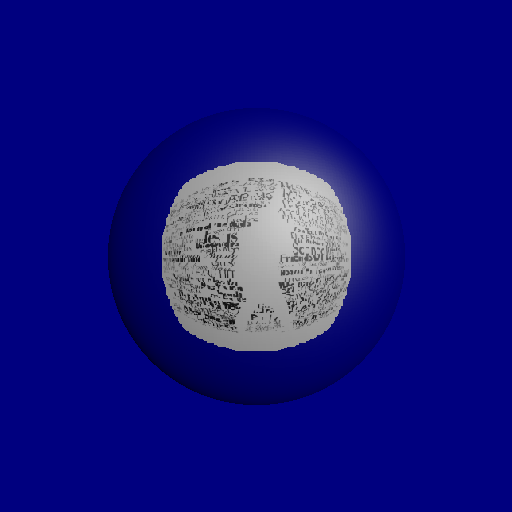
\includegraphics[width=\linewidth]{images/spere_mirror_high_lod_linear}
		\caption{Linear Interpolation.}
	\end{subfigure}
	\begin{subfigure}[b]{0.49\linewidth}
		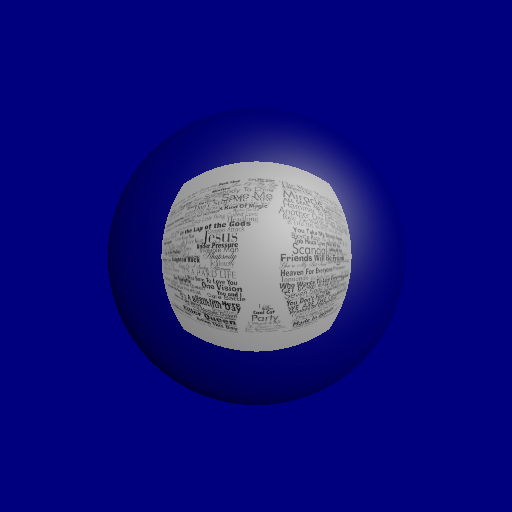
\includegraphics[width=\linewidth]{images/spere_mirror_high_lod_cubic}
		\caption{Cubic Interpolation.}
	\end{subfigure}
	\caption{Reflective sphere scene with mipmapping, $\testhighres^3$ grid dimension, linear vs cubic interpolation comparison.}
	\label{fig:testlowinterpolation}
\end{figure}

\begin{figure}[H]
	\centering
	
\includegraphics[width=0.6\linewidth]{images/spere_mirror_high_lod_cubic_ssaa}
	\caption{Reflective sphere scene with mipmapping, $\testhighres^3$ grid dimension, cubic interpolation, 2x SSAA.}
	\label{fig:testssaa}
\end{figure}

\section{Conclusion}
Summarizing, a general definition of discrete signed distance fields can be formulated to successfully make use ray differentials to estimate the footprint of a ray in the scenes. Arbitrary interpolation kernels can be used for the signed distance function although higher order kernels are recommendable to avoid blocky looking curved shapes. The use of higher order kernels may also produce good results with a low grid resolution which lowers the memory consumption. Using ray differentials for estimating the footprint on a texture is an effective way to reduce aliasing when mapping textures to signed distance fields. Another practical use of ray differentials with signed distance functions may be choosing LoD levels of the voxel grid itself to filter among different detail representations of the scene or certain objects. 

%\section{Voxel Ray Differentials}

\subsection{Signed Distance Function and Trilinear Interpolation}
Our discrete Signed Distance Function is defined by trilinear filtering over discrete grid values. To calculate the value of the Signed Distance Function given a world position, we first have to project the world position to the local voxel grid. This can be done using the following equation to convert the world position $P_{w}$ into a voxel gird coordinate $P_{grid} \in [0, V_{resolution}]$.
\begin{equation}
P_{grid} = V_{resolution} \left(\frac{\left(P_{w} - V_{origin}\right)}{2V_{scale}}  + \begin{pmatrix}\frac{1}{2} & \frac{1}{2} & \frac{1}{2}\end{pmatrix}^T \right) 
\end{equation}
$V_{origin}$ and $V_{scale}$ represent the origin and the scale of the voxel grid, $V_{resolution}$ is its resolution.

For performing the trinilear interpolation, the 8 neighbor cells of the specific position have to be obtained. The filter weight $t$, respective to lowest cell, has to be calculated.

\begin{figure}[H]
	\caption{Trilinear filter weight $t$ to weight the 8 respective neighbor cells}
	\centering
	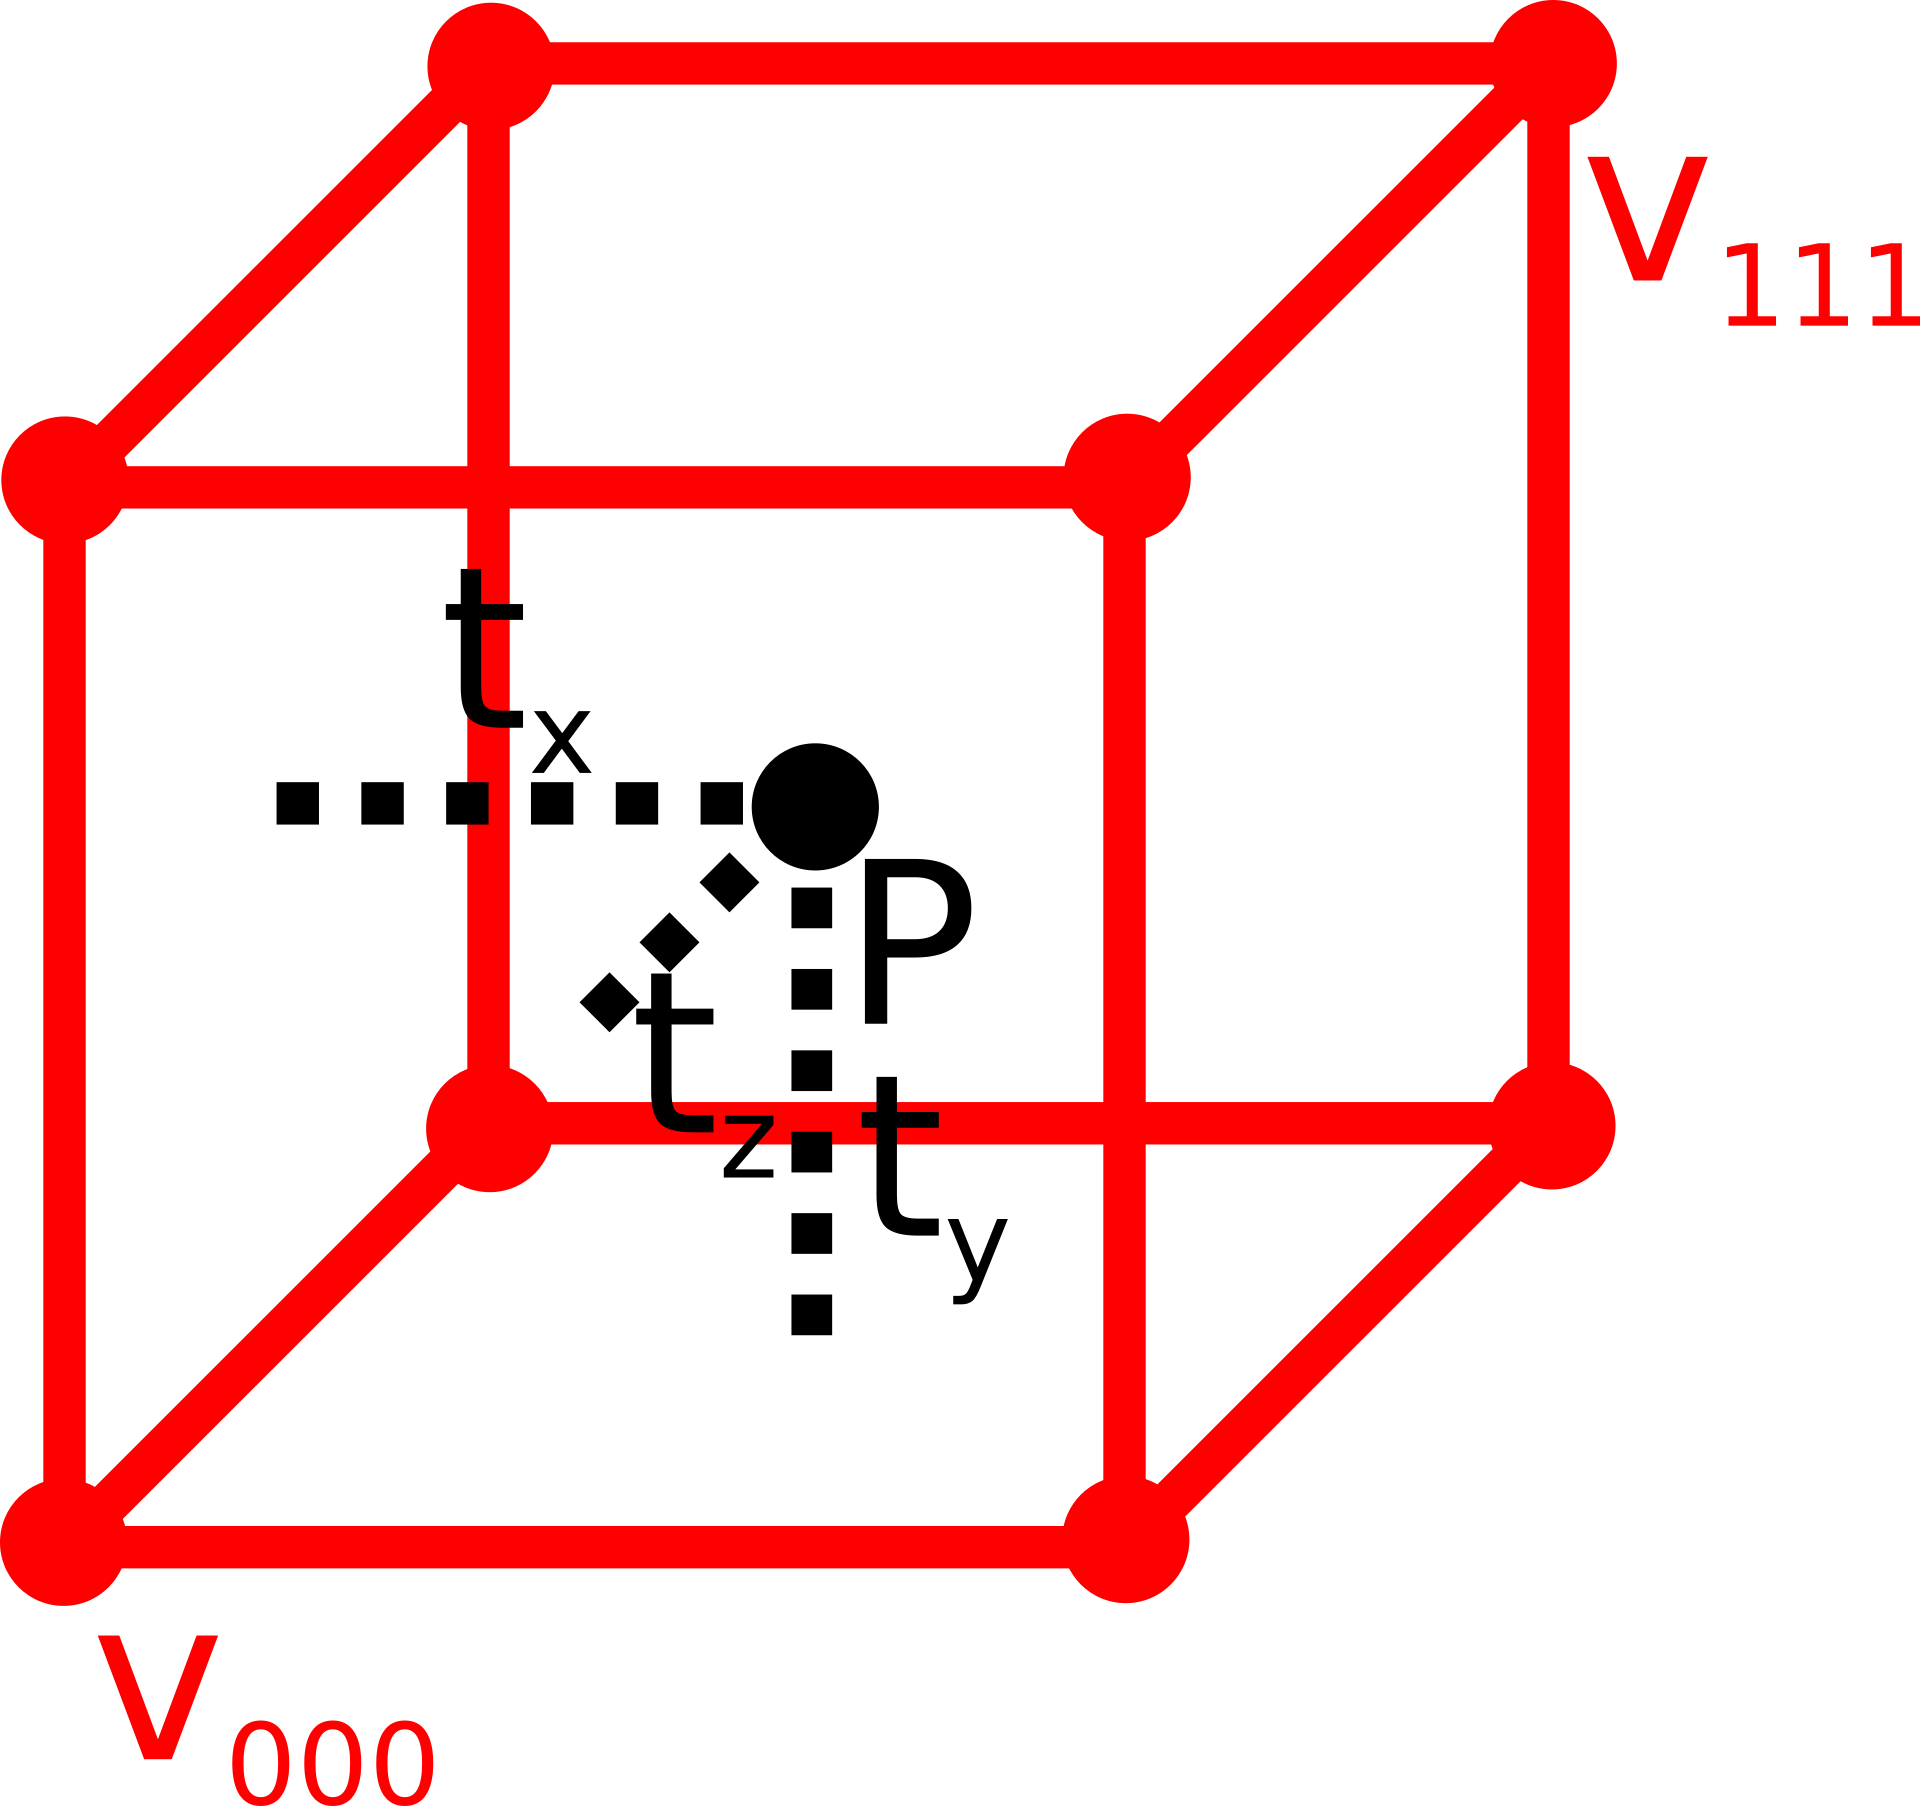
\includegraphics[width=10em]{images/trilinear_filter_weight}
\end{figure}
\begin{equation}
t = P_{grid} - P_{000}
\end{equation}
Since the width of a cell is 1, no division has to be done.

The final step is to build the filter matrix $T$ and calculate its dot product with the 8 neighbor cells. This yields the interpolated value at $P_{grid}$, the value of the Signed Distance Function.

\begin{equation}
T =
\begin{pmatrix}
(1 - t_x) (1 - t_y) (1 - t_z) \\
t_x (1 - t_y) (1 - t_z) \\
(1 - t_x) t_y (1 - t_z) \\
(1 - t_x) (1 - t_y) t_z \\
t_x t_y (1 - t_z) \\
t_x (1 - t_y) t_z \\
(1 - t_x) t_y t_z \\
t_x t_y t_z
\end{pmatrix}	
V =
\begin{pmatrix}
v_{000} \\
v_{100} \\
v_{010} \\
v_{001} \\
v_{110} \\
v_{101} \\
v_{011} \\
v_{111} 
\end{pmatrix}
, trilinear(t, V) = T \cdot V
\end{equation}

\begin{equation}
SDF(P) = trilinear(t_P, V_{sdf})
\end{equation}

\subsection{Surface Normal}

The surface of the Signed Distance Function is defined as the set of points where the Signed Distance Function yields 0.
\begin{equation}
S_{surface} = \{P \in \mathbb{R}^3 \mid SDF(P) = 0\}
\end{equation}
For $P \in S_{surface}$, the surface normal $N$ is defined as the gradient of the Signed Distance Field.

\begin{equation}
n_{surface} = \nabla SDF = 
\begin{pmatrix}
\pardiff{trilinear(t_P, V_{sdf})}{x_{w}} \newlinell
\pardiff{trilinear(t_P, V_{sdf})}{y_{w}} \newlinell
\pardiff{trilinear(t_P, V_{sdf})}{z_{w}}
\end{pmatrix}
\end{equation}
$\partial x_{w}$, $\partial y_{w}$ and $\partial z_{w}$ denotes the differential in world coordinates, a change in the x, y and z-axis. To calculate the gradient of the Signed Distance Function, the trilinear interpolation has to be differentiated. For the x-direction, the differential of the trilinear filter weight $t$ is a constant value depending on the scale and resolution of the grid

\begin{equation}
\pardiff{P_w}{x_w} = 
\begin{pmatrix}
1 & 0 & 0
\end{pmatrix}^T
\qquad
\pardiff{t}{x_w} = 
\frac{V_{resolution}}{2V_{scale}}
\begin{pmatrix}
1 & 0 & 0
\end{pmatrix}^T.
\end{equation}
This results in the following equation for the differential of the trilinear interpolation in x-direction.

\begin{equation}
\pardiff{trilinear(t_P, V_{sdf})}{x_{w}} = 
\frac{V_{resolution}}{2V_{scale}}
V_{sdf} \cdot
\begin{pmatrix}
-(1 - t_y) (1 - t_z) \newlinel
(1 - t_y) (1 - t_z) \newlinel
-t_y (1 - t_z) \newlinel
-(1 - t_y) t_z \newlinel
t_y (1 - t_z) \newlinel
(1 - t_y) t_z \newlinel
-t_y t_z \newlinel
t_y t_z
\end{pmatrix}
\end{equation}
A similar expression can be derived for the y and z-direction. Final normalization results in the surface normal

\begin{equation}
N_{surface} = \frac{n_{surface}}{\left(n_{surface} \cdot n_{surface}\right)^{1/2}} .
\end{equation}

\subsubsection{Surface Normal Differentials}
To use ray differentials with voxel based objects, the surface normal has to be differentiated by the image plane coordinates $x$ and $y$.
\begin{equation}
\pardiffx{n_{surface}} = 
\begin{pmatrix}
\pardiffsq{trilinear(t_P, V_{sdf})}{x_{w}}{x} \newlinell
\pardiffsq{trilinear(t_P, V_{sdf})}{y_{w}}{x} \newlinell
\pardiffsq{trilinear(t_P, V_{sdf})}{z_{w}}{x}
\end{pmatrix}
\qquad
\pardiffy{n_{surface}} = 
\begin{pmatrix}
\pardiffsq{trilinear(t_P, V_{sdf})}{x_{w}}{y} \newlinell
\pardiffsq{trilinear(t_P, V_{sdf})}{y_{w}}{y} \newlinell
\pardiffsq{trilinear(t_P, V_{sdf})}{z_{w}}{y}
\end{pmatrix}
\end{equation}
The differential of the interpolation weight $t$ by the image plane coordinates based on the ray differential positions $\pardiffx{P}$ and $\pardiffy{P}$ is
\begin{equation}
\pardiff{t}{x} = \frac{V_{resolution}}{2V_{scale}} \pardiff{P}{x}
\qquad
\pardiff{t}{y} = \frac{V_{resolution}}{2V_{scale}} \pardiff{P}{y}.
\end{equation}
This yields the following term for the x-coordinate of the $\partial x$ normal differential $\pardiffx{n_{surface}}$
\begin{equation}
\pardiffsq{trilinear(t_P, V_{sdf})}{x_{w}}{x} = 
\left(\frac{V_{resolution}}{2V_{scale}}\right)^2
V_{sdf}
\cdot
\left(
\begin{pmatrix}
\pardiffx{P_y} (1 - t_z) \newlinel
-\pardiffx{P_y} (1 - t_z) \newlinel
-\pardiffx{P_y} (1 - t_z) \newlinel
\pardiffx{P_y} t_z \newlinel
\pardiffx{P_y} (1 - t_z) \newlinel
-\pardiffx{P_y} t_z \newlinel
-\pardiffx{P_y} t_z \newlinel
\pardiffx{P_y} t_z
\end{pmatrix}
+
\begin{pmatrix}
(1 - t_y) \pardiffx{P_z} \newlinel
-(1 - t_y) \pardiffx{P_z} \newlinel
t_y \pardiffx{P_z} \newlinel
-(1 - t_y) \pardiffx{P_z} \newlinel
-t_y \pardiffx{P_z} \newlinel
(1 - t_y) \pardiffx{P_z} \newlinel
-t_y \pardiffx{P_z} \newlinel
t_y \pardiffx{P_z}
\end{pmatrix}
\right).
\end{equation}
All other 5 components can be derived regarding this expression. To retrieve the normalized normal differential, the normalization term has to be derived to receive
\begin{equation}
\pardiffx{N} = \frac{(n \cdot n) \pardiffx{n} - (n \cdot \pardiffx{n}) n}{(n \cdot n)^{3/2}}
\end{equation}

\subsection {Shading Normal}
Using surface normals produces hard edges on voxel borders which reveals the block structure. To avoid this problem, trilinear interpolation of the surface normals can be applied to receive a smooth normal at a given point.
\begin{equation}
n = trilinear(t_p, V_{N_{surface}})
\end{equation}
where $V_{N_{surface}}$ is an 8-compoment vector consisting of the surface normals of the 8 neighbor cells of the respective position.
\subsubsection {Shading Normal Differential}
The differential of the shading normal requires the differential of the trilinear equation. For the $\partial x$ differential this would be
\begin{equation}
\pardiffx{n} = \pardiffx{trilinear(t_p, V_{N_{surface}})} = \pardiffx{T} \cdot V_{N_{surface}}
\end{equation}

\begin{equation}
\begin{aligned}
\pardiffx{T} &=
\begin{pmatrix}
\left(-\pardiffx{t_x}\right) (1 - t_y) (1 - t_z) \newlinel
\pardiffx{t_x} (1 - t_y) (1 - t_z) \newlinel
\left(-\pardiffx{t_x}\right) t_y (1 - t_z) \newlinel
\left(-\pardiffx{t_x}\right) (1 - t_y) t_z \newlinel
\pardiffx{t_x} t_y (1 - t_z) \newlinel
\pardiffx{t_x} (1 - t_y) t_z \newlinel
\left(-\pardiffx{t_x}\right) t_y t_z \newlinel
\pardiffx{t_x} t_y t_z
\end{pmatrix}
+
\begin{pmatrix}
(1 - t_x) \left(-\pardiffx{t_y}\right) (1 - t_z) \newlinel
t_x \left(-\pardiffx{t_y}\right) (1 - t_z) \newlinel
(1 - t_x) \pardiffx{t_y} (1 - t_z) \newlinel
(1 - t_x) \left(-\pardiffx{t_y}\right) t_z \newlinel
t_x \pardiffx{t_y} (1 - t_z) \newlinel
t_x \left(-\pardiffx{t_y}\right) t_z \newlinel
(1 - t_x) \pardiffx{t_y} t_z \newlinel
t_x \pardiffx{t_y} t_z
\end{pmatrix}
\\
&+
\begin{pmatrix}
(1 - t_x) (1 - t_y) \left(-\pardiffx{t_z}\right) \newlinel
t_x (1 - t_y) \left(-\pardiffx{t_z}\right) \newlinel
(1 - t_x) t_y \left(-\pardiffx{t_z}\right) \newlinel
(1 - t_x) (1 - t_y) \pardiffx{t_z} \newlinel
t_x t_y \left(-\pardiffx{t_z}\right) \newlinel
t_x (1 - t_y) \pardiffx{t_z} \newlinel
(1 - t_x) t_y \pardiffx{t_z} \newlinel
t_x t_y \pardiffx{t_z}
\end{pmatrix}
\end{aligned}
\end{equation}

\subsection{New Section}
1D kernel with kernel width $n$
\begin{equation}
f(v_0, \dots, v_{n-1}, t)
\end{equation}
Linear filter kernel example
\begin{equation}
f(v_0, v_1, t) = (1 - t) v_0 + t v_1
\end{equation}
Applying kernel with width $2$ to 3D voxel grid
\begin{equation}
%f(f(f(v0, v1, t_x(P)), f(v2, v3, t_x(P)), t_y(P)), f(f(v4, v5, t_x(P)), f(v6, v7, t_x(P)), t_y(P)), t_z(P))
v(t) = f
\begin{pmatrix}
f 
\begin{pmatrix}
f(v0, v1, t_x), \\
f(v2, v3, t_x), \\
t_y
\end{pmatrix}, \\[2.0em]
f
\begin{pmatrix}
f(v4, v5, t_x), \\
f(v6, v7, t_x), \\
t_y
\end{pmatrix}, \\[2.0em]
t_z
\end{pmatrix}
\end{equation}
\begin{equation}
SDF(P) = v(t(P))
\end{equation}
Normal
\begin{equation}
n = \nabla SDF = 
\begin{pmatrix}
\pardiff{SDF}{P_x} \newlinell
\pardiff{SDF}{P_y} \newlinell
\pardiff{SDF}{P_z}
\end{pmatrix}
=
\begin{pmatrix}
\pardiff{v}{t_x} \newlinell
\pardiff{v}{t_y} \newlinell
\pardiff{v}{t_z}
\end{pmatrix}
\odot
\begin{pmatrix}
\pardiff{t_x}{P_x} \newlinell
\pardiff{t_y}{P_y} \newlinell
\pardiff{t_z}{P_z}
\end{pmatrix}
=
\nabla v \odot \pardiff{t}{P}
\end{equation}
Normal Differentials
\begin{equation}
\begin{aligned}
\pardiff{n}{x} &= \pardiff{\nabla SDF}{x} = 
\begin{pmatrix}
\pardiffsq{SDF}{P_x}{x} \newlinell
\pardiffsq{SDF}{P_y}{x} \newlinell
\pardiffsq{SDF}{P_z}{x}
\end{pmatrix} \newlinell
&=
\begin{pmatrix}
\pardiffsqsame{v}{t_x} \pardiff{t_x}{P_x} \pardiff{P_x}{x} + \pardiffsq{v}{t_x}{t_y} \pardiff{t_y}{P_y} \pardiff{P_y}{x} + \pardiffsq{v}{t_x}{t_z} \pardiff{t_z}{P_z} \pardiff{P_z}{x} \newlinell
\pardiffsq{v}{t_y}{t_x} \pardiff{t_x}{P_x} \pardiff{P_x}{x} + \pardiffsqsame{v}{t_y} \pardiff{t_y}{P_y} \pardiff{P_y}{x} + \pardiffsq{v}{t_y}{t_z} \pardiff{t_z}{P_z} \pardiff{P_z}{x} \newlinell
\pardiffsq{v}{t_z}{t_x} \pardiff{t_x}{P_x} \pardiff{P_x}{x} + \pardiffsq{v}{t_z}{t_y} \pardiff{t_y}{P_y} \pardiff{P_y}{x} + \pardiffsqsame{v}{t_z} \pardiff{t_z}{P_z} \pardiff{P_z}{x}
\end{pmatrix}
\odot \pardiff{t}{P} \newlinell
&=
\begin{pmatrix}
\pardiffsqsame{v}{t_x} & \pardiffsq{v}{t_x}{t_y} & \pardiffsq{v}{t_x}{t_z} \newlinell
\pardiffsq{v}{t_y}{t_x} & \pardiffsqsame{v}{t_y} & \pardiffsq{v}{t_y}{t_z} \newlinell
\pardiffsq{v}{t_z}{t_x} & \pardiffsq{v}{t_z}{t_y} & \pardiffsqsame{v}{t_z}
\end{pmatrix}
\cdot \left( \pardiff{t}{P} \odot \pardiff{t}{P} \odot \pardiff{P}{x} \right) \newlinell
&= \Hessian(v) \cdot \left(\pardiff{t}{P} \odot \pardiff{t}{P} \odot \pardiff{P}{x} \right)
\end{aligned}
\end{equation}


\printbibliography 

\end{document}
  